\chapter{Теоретическая часть}

\section{ПРИМЕЧАНИЕ для проверяющих отчёт по практике}

\textit{[В чистовом тексте этого раздела не будет]}

\begin{figure}
  \centering
  \includegraphics[width=0.5\textwidth]{inc/img/ugra-moscow}
  \caption{Ugra CTF School 2022. Долгопрудный}
\end{figure}

Я прохожу практику в Югорском научно-исследовательском институте информационных технологий. В мои обязанности входит разработка и проведение школьной олимпиады по информационной безопасности Ugra CTF. Я разрабатываю систему, состоящую из двух компонент:

\begin{enumerate}
\item веб-приложения Kyzylborda, выдающего участникам материалы олимпиады и проверяющее их решения с технологией защиты от списывания;
\item дистрибутива GNU/Linux SchoolOS, рассчитанный на Live-загрузку с переносного носителя, который обладает следующей функциональностью:
  \begin{enumerate}
  \item Автоматически разворачивается виртуальная машина с образом любой ОС, предоставленной каждым участником;
  \item Из того же личного кабинета подтягиваются данные участника: известно за какой машиной под каким номером кто сидит;
  \item Все остальные приложения полностью изолируются от участника;
  \item Реализованы элементы прокторинга: периодически с машины каждого участника собираются скриншоты, которые в перспективе планируется автоматически анализировать на предмет нарушения правил — там всё неочевидно, поскольку мы разрешаем пользоваться интернетом, но запрещаем любую внешнюю помощь и распространение условий задач;
  \item Обеспечивается возможность удалённого доступа организаторов к любой машине;
  \item Гарантируется невозможность модификации запущенной хост-ОС: её системных файлов, конфигурации ПО и пользователей с группами.
  \end{enumerate}
\end{enumerate}

Система основана она на функциональном пакетном менеджере Nix, прелесть которого в том, что желаемое состояние ОС можно описать декларативно. Nix выполнит оптимальный набор действий, который приведёт систему в это состояние, причём изменять его иначе нельзя никак — пути до исполняемых и конфигурационных файлов суть ссылки до read-only хранилища. Остальные компоненты системы планируется реализовать с помощью смеси bash- и Python-скриптов, а также централизованной проверяющей системы — веб-приложения с API.

\begin{figure}
  \centering
  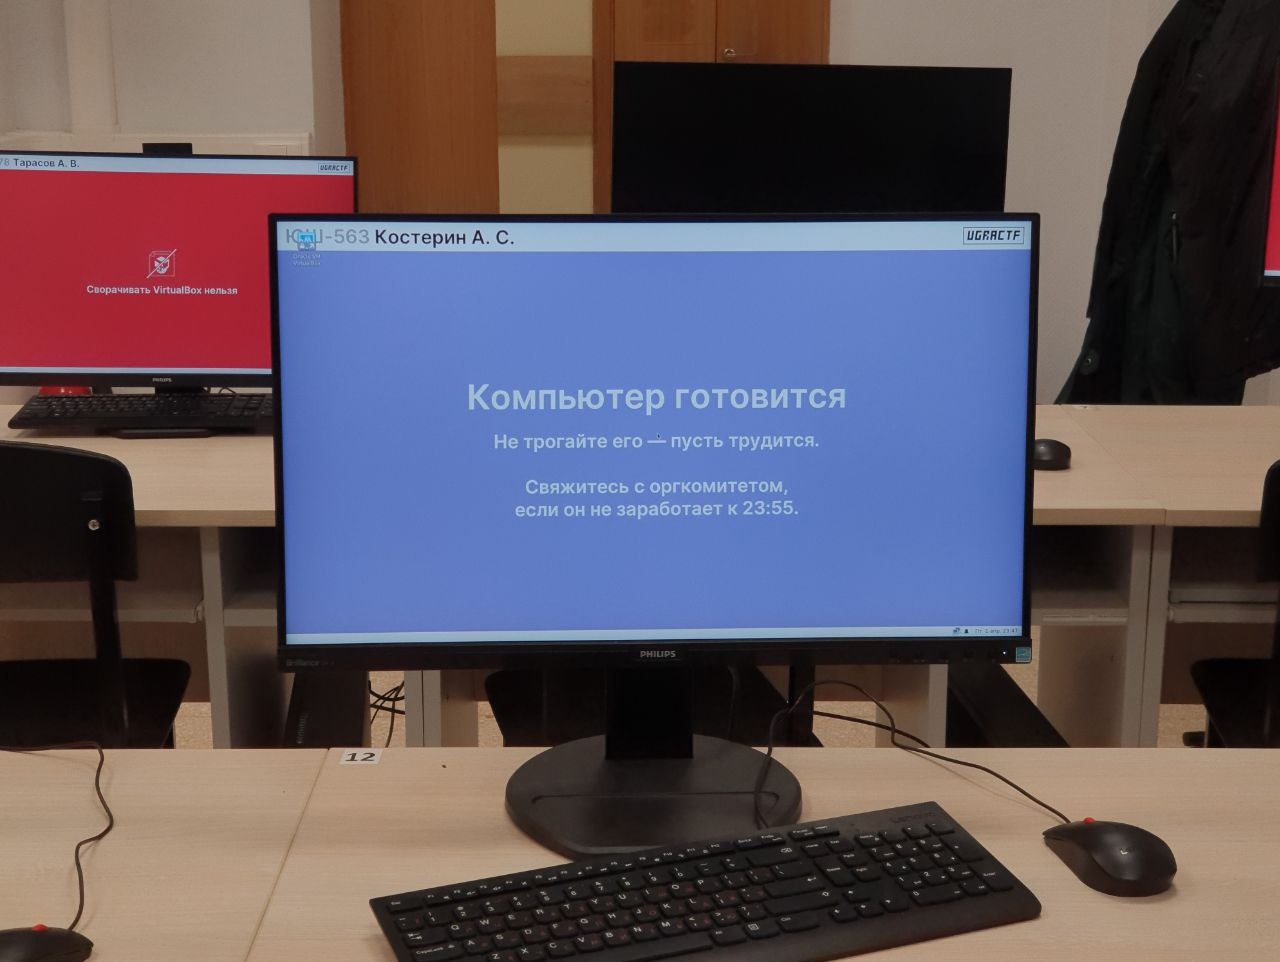
\includegraphics[width=0.5\textwidth]{inc/img/ugra-schoolos}
  \caption{Инициализация аудитории с 10 рабочими станциями с помощью SchoolOS. Долгопрудный, за день до олимпиады}
\end{figure}

2 апреля 2022 года мы с коллегами провели испытание системы, разработке которой посвящена данная ВКР, во время проведения всероссийской олимпиады школьников по защите информации Ugra CTF School 2022.

Система практически без проблем одновременно запустилась на более чем сорока компьютерах на площадках нашей олимпиады по всей стране: в Санкт-Петербурге, Долгопрудном, Красноярске, Тюмени, Екатеринбурге, Сургуте, Ханты-Мансийске, Новосибирске, Перми и Владивостоке.

\begin{figure}
  \centering
  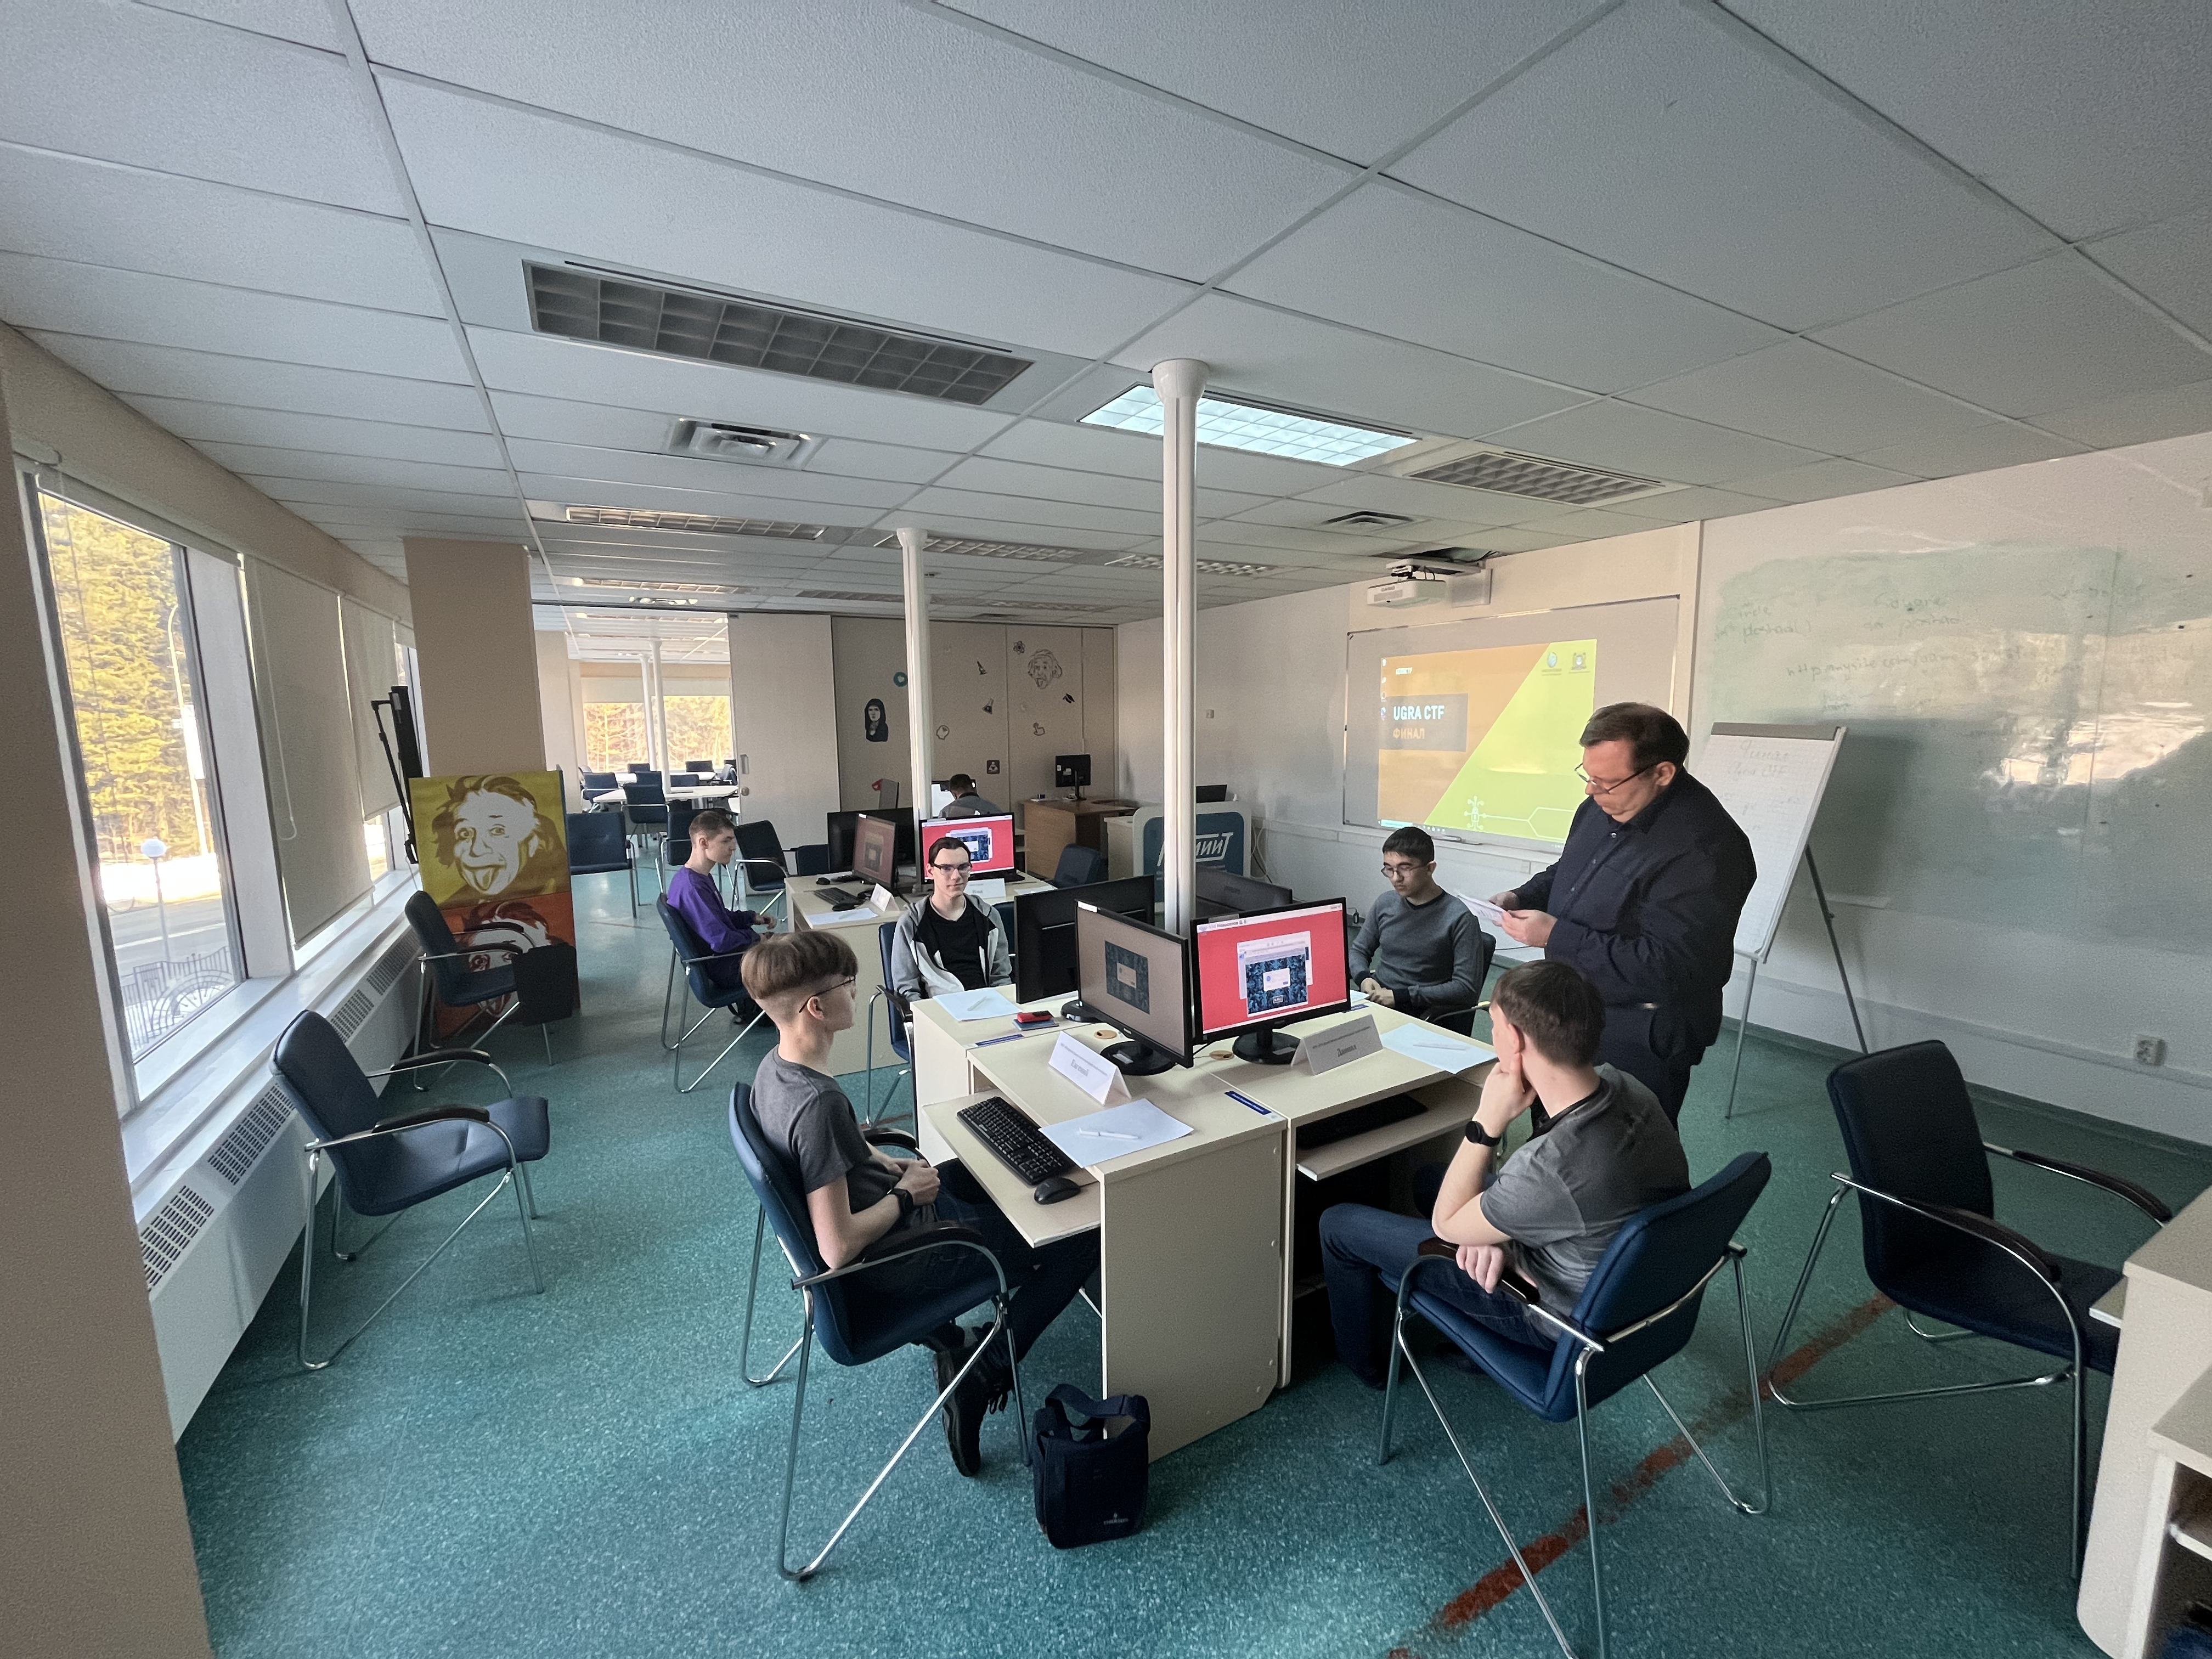
\includegraphics[width=0.5\textwidth]{inc/img/ugra-hm}
  \caption{Ugra CTF School 2022. Ханты-Мансийск}
\end{figure}

В Долгопрудном, на площадке Московского физико-технического института, я лично наблюдал за ходом олимпиады и работой системы. Всё прошло как планировалось: все компьютеры загрузились, подключились к интернету и нашей проверяющей системе, автоматически получили соответствующие данные об участниках и проинициализировали образы виртуальных машин, за которыми детям и
предстояло решать тур олимпиады.

\begin{figure}
  \centering
  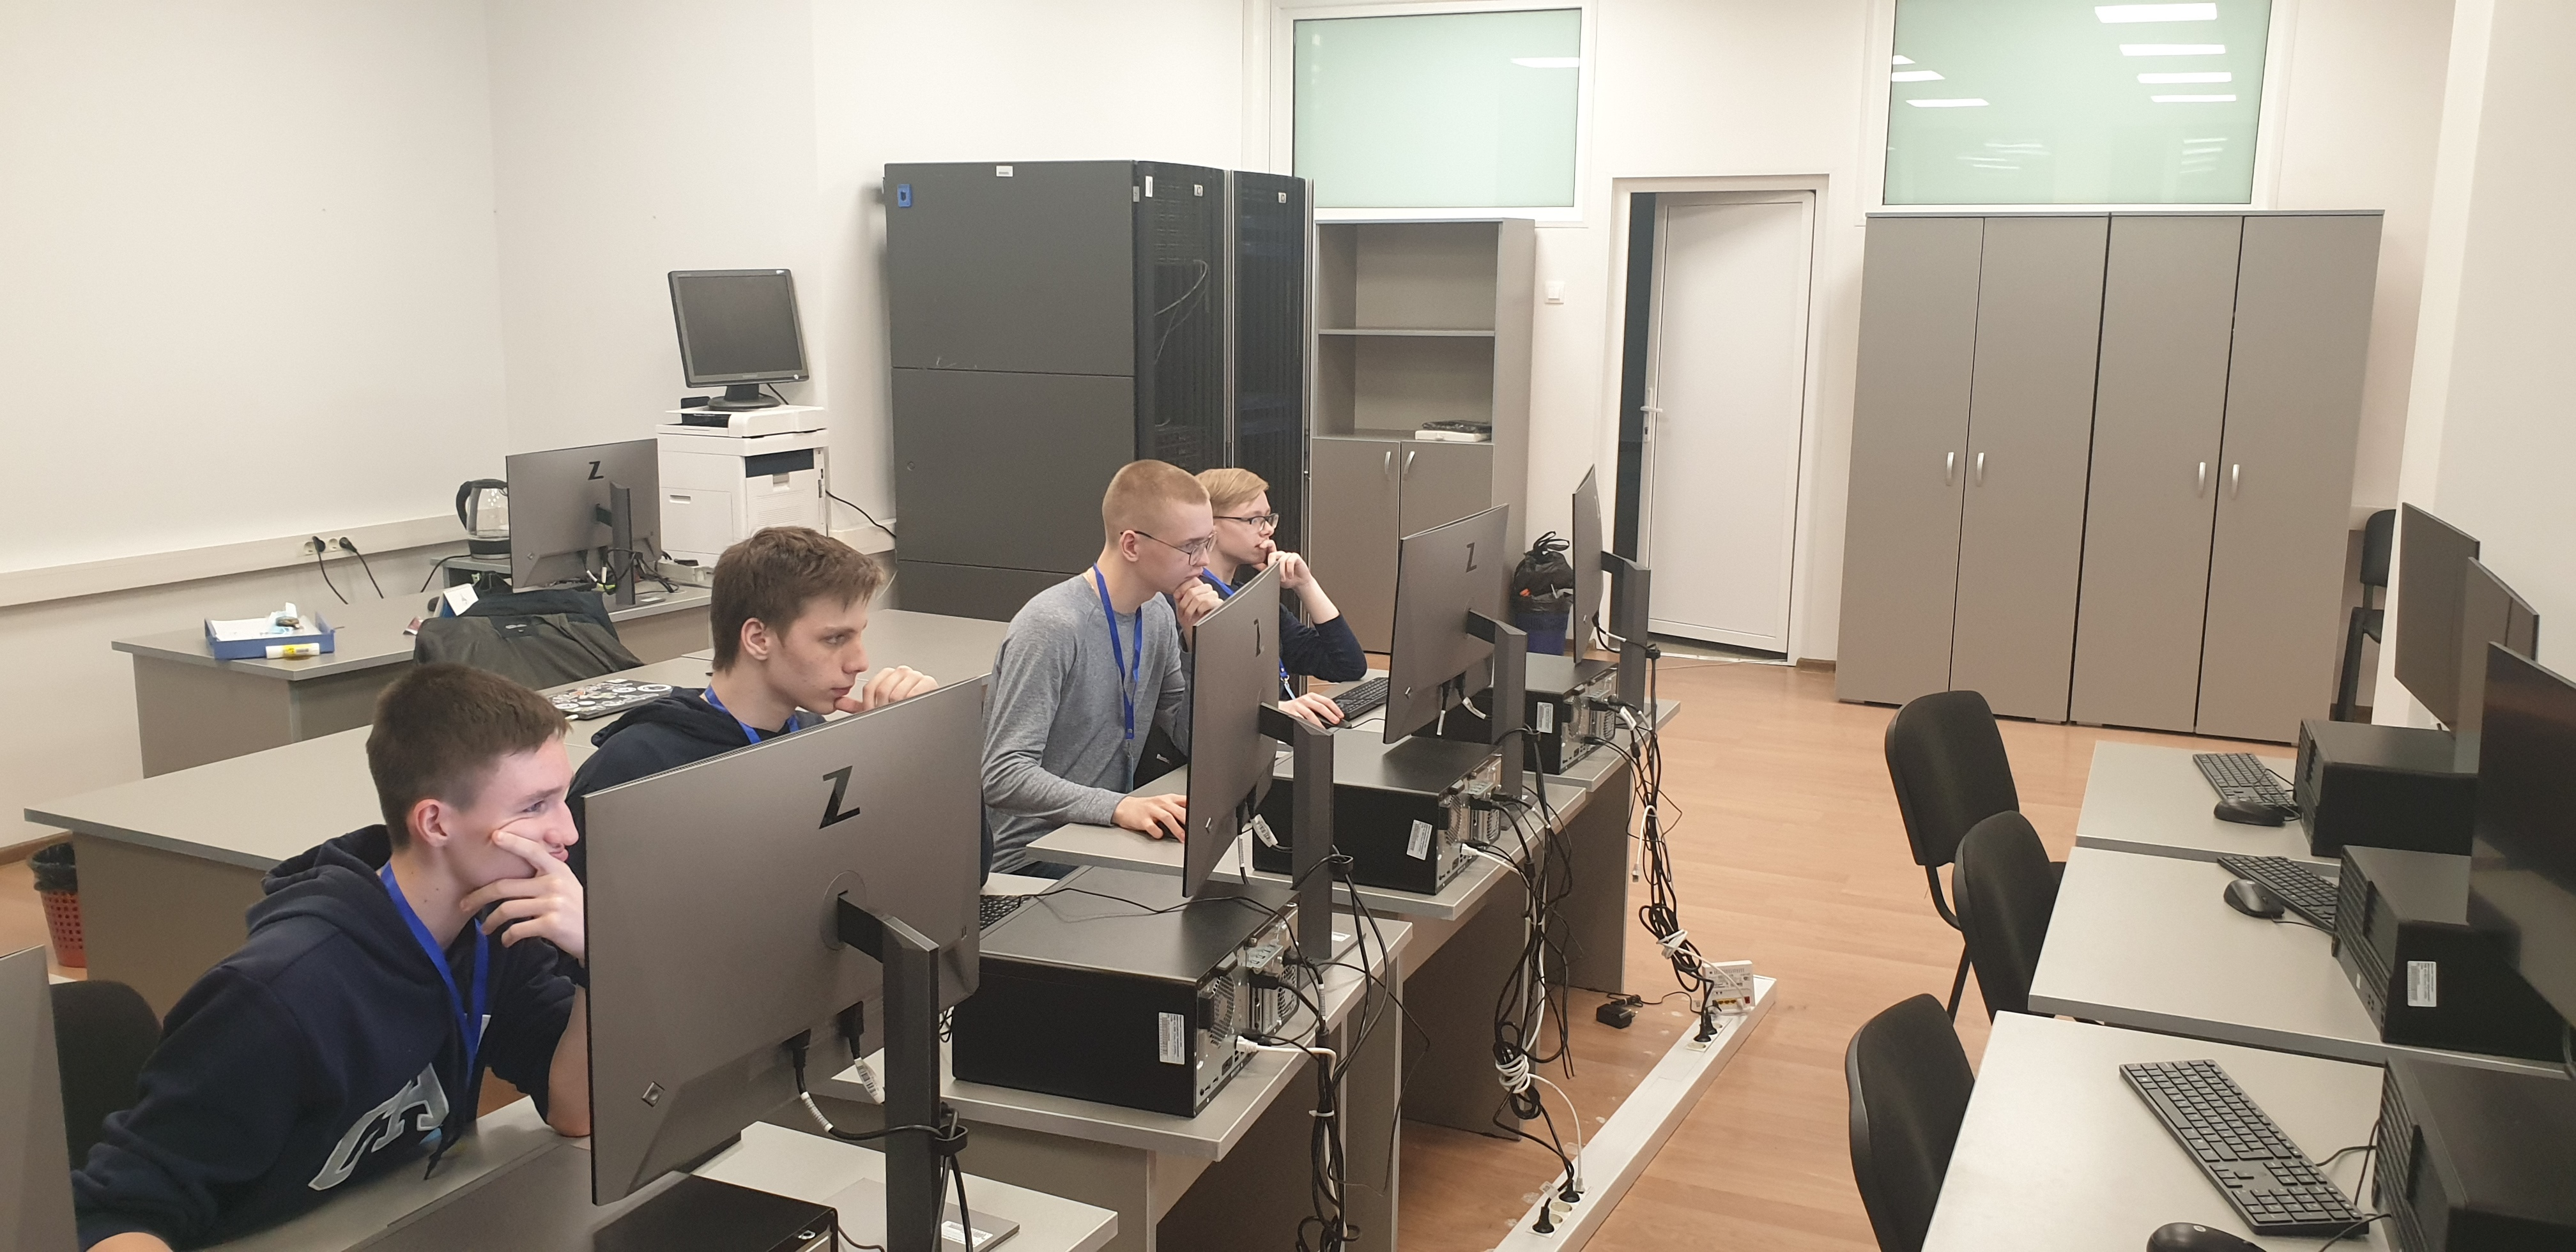
\includegraphics[width=0.5\textwidth]{inc/img/ugra-vladivostok}
  \caption{Ugra CTF School 2022. Владивосток}
\end{figure}

Это мероприятие по большому счёту проводится силами всего четырёх человек, включая меня, а рабочих задач \textit{очень} много. Кроме разработки системы и участия в проведении олимпиады я помогал организовать вышеупомянутую площадку в МФТИ, а в настоящий момент мы с коллегами составляем отчётную документацию для Российского совета олимпиады школьников, а также занимаемся логистикой призов победителям и призёром в непростых экономических условиях.

Всё это отрицательно сказалось на объёме текста ВКР, который был мной написан. Я обещаю оперативно исправиться и предоставить чистовую версию данного отчёта не позднее середины следующей недели.

Текст ниже --- черновой.

\begin{figure}
  \centering
  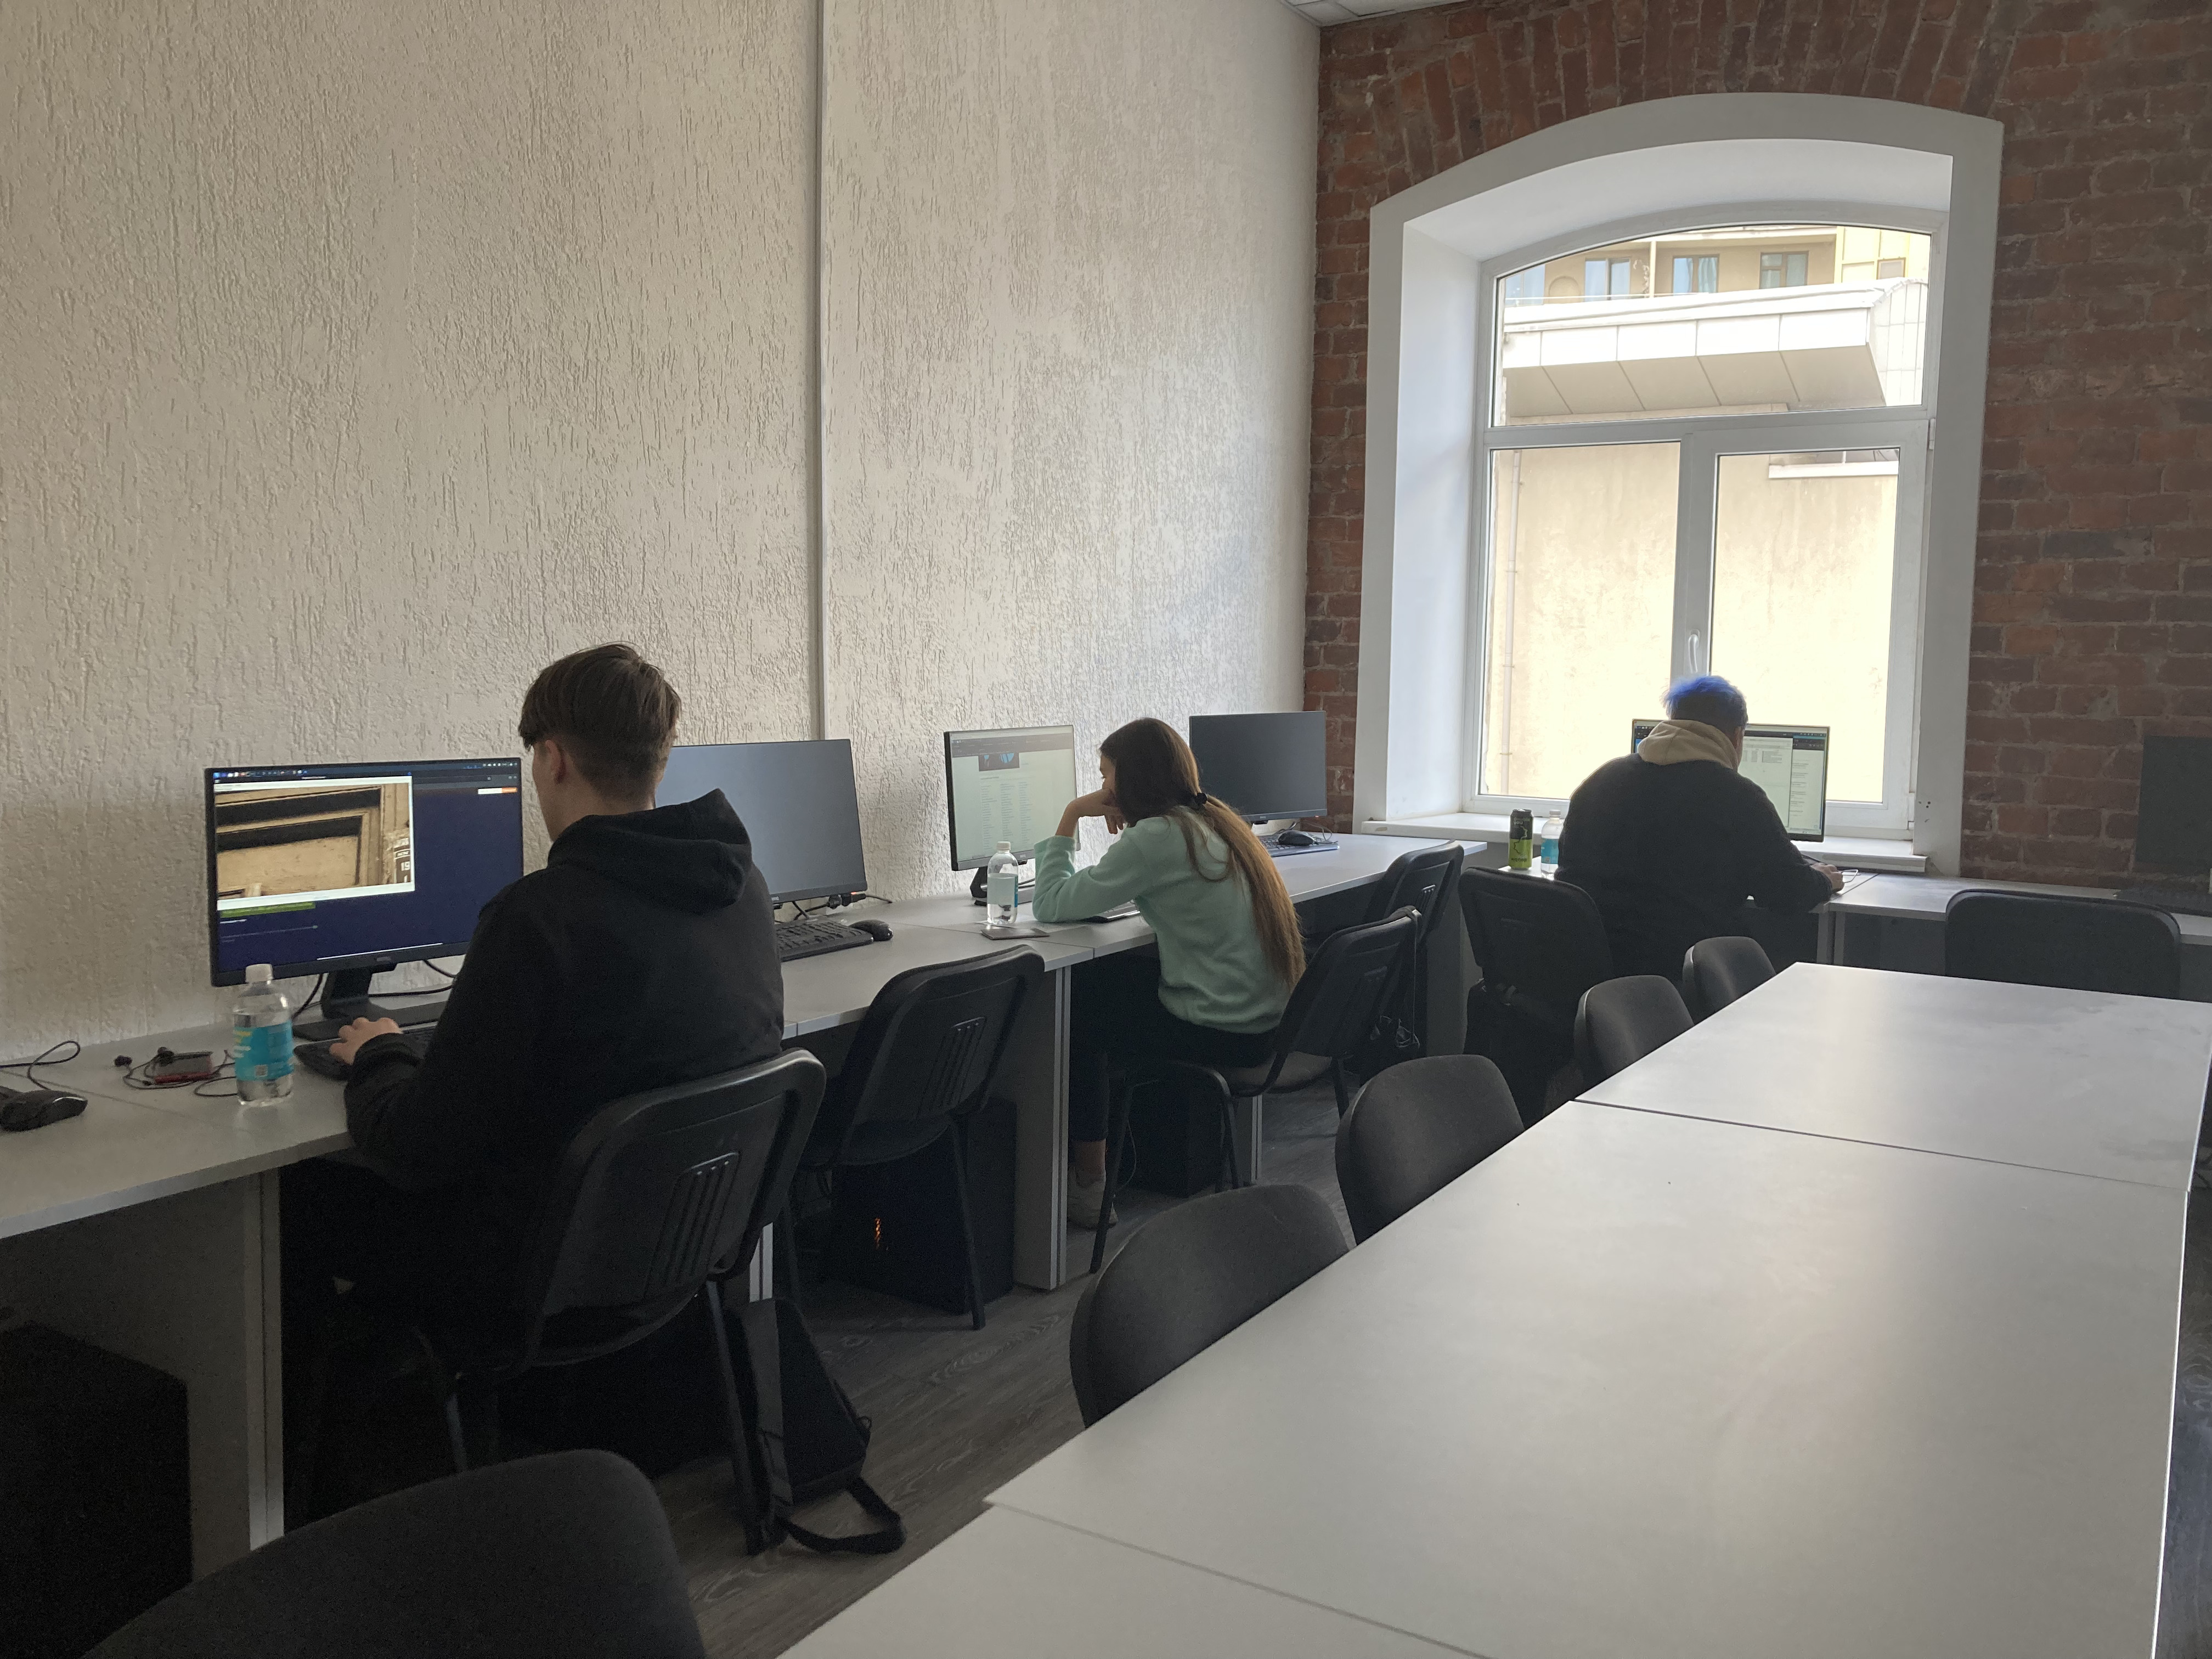
\includegraphics[width=0.5\textwidth]{inc/img/ugra-spb}
  \caption{Ugra CTF School 2022. Санкт-Петербург}
\end{figure}

\section{Техническая архитектура соревнований}

Автоматизированный подход применён для решения трёх основных задач.

Управление материалами соревнований (включая тексты задач, приём и проверку решений, подведение итогов, а также определение попыток списывания).

Предоставлене среды для решения заданий участниками. Система SchoolOS.

Прокторинг.


%% Для проведения соревнований Ugra CTF необходима комплексная архитектура, которая позволит решить следующие задачи:

%% \begin{enumerate}

%% \item обеспечение решения игровых задач, включая получение условий, приём, валидацию и проверку флагов;
%% \item

%% \end{enumerate}

%% \Abbrev{TCP}{transmission control protocol --- протокол управления передачей}

\subsection{Система, обеспечивающая решение игровых задач}

Соревнования вида jeopardy с самого начала были автоматизированы. Это связано с относительно более тривиальным игровым процессом, чем в соревнованиях вида attack-defense. Обычно участники получают доступ к веб-приложению, которое содержит условия задач, турнирную таблицу и форму для сдачи флага. Его принято называть бордой.

\Define{борда}{\textit{(англ. board, буквально «доска»)} --- программная платформа для получения условий задач и сдачи флагов в CTF-соревнованиях вида jeopardy.}


\subsubsection{Требования к системе}

Борда должна отвечать ряду требований.

\begin{enumerate}

\item
В первую очередь, к таким требованиям можно отнести устойчивость к высоким нагрузкам. В отличие от соревнований вида attack-defense, где нагрузка команды атакуют друг друга (отношение «многие ко многим»), в jeopardy участники взаимодействуют с централизованной игровой инфраструктурой организаторов (отношение «многие к одному»). Отказ в обслуживании со стороны игровой платформы категорически недопустим, поскольку он создаёт неравные условия для игроков: возможна ситуация, когда часть участников успеет получить условие задачи или сдать флаг, в то время как другая --- нет.

Основные операции в платформе должны выполняться быстро и без существенных задержек. Желательно, чтобы система поддерживала многопоточную обработку пользовательских запросов там, где это возможно.

\item
Многопоточность, однако, зачастую приводит к неопределённости параллелизма. Эта неопределённость может послужить причиной ошибок: двойному начислению баллов, списанию некорректной суммы баллов при взятии подсказок или достижению некорректного состояния системы.

\Define{Неопределённость параллелизма}{ошибка проектирования многопоточной системы или приложения, при которой работа системы или приложения зависит от того, в каком порядке выполняются части кода}

\item
Тот факт, что соревнования --- по защите информации, накладывают повышенные требования к безопасности платформы. Не смотря на то, что правилами Ugra CTF запрещены атаки на инфраструктуру, непосредственно не относящуюся к игровым задачам, попытки вывести её из строя всё равно предпринимаются. Система должна быть устойчивой к наиболее распространённым веб-уязвимостям (обработка запросов, контроль пользовательских сессий и проч.), а также вести аудит всех событий для своевременного обнаружения оргкомитетом новых угроз.

\item
Платформа должна позволять обнаружать не только технические угрозы, но и более «человеческие»: пресекать попытки списывания, обмена участников флагами, решения соревнований одним и тем же лицом с нескольких аккаунтов (т.е. мультиаккаунтинг).

\item
Наконец, система должна быть гибкой. CTF --- творческий формат, поэтому структура и принципы могут меняться от игры к игры. Так, отборочный этап Ugra CTF 2019 представлял собой не простой jeopardy, где участникам сразу доступны все задания, а модельный тест на проникновение: сперва игрокам доступна лишь одна точка входа в вымышленную уязвимую систему. По мере «погружения» влубь этой системы открывались новые задания, которые выстраивались в нелинейную древовидную структуру\cite{UgraCTF19Q}.
\end{enumerate}


\subsubsection{Анализ существующих решений}

Существует множество программных продуктов, позволяющих проводить jeopardy -- CTF-соревнования, что называется, «под ключ»: организаторам необходимо лишь собрать участников, разработать задания и загрузить их на готовую платформу, при необходимости изменив некоторые её параметры. К сожалению, автору не удалось обнаружить такой системы, которая удовлетворяла бы всем требованиям \textit{(а)---(д)}, данным выше (табл. \ref{tab:boards}).

\begin{center}
  \begin{longtable}{|p{0.26\textwidth}|p{0.15\textwidth}|p{0.25\textwidth}|c|c|c|c|c|}
    \caption{Сравнительный анализ наиболее популярных готовых jeopardy-платформ}
    \label{tab:boards}
    \\ \hline
    \multirow{2}{*}{Название} & \multirow{2}{*}{Лицензия} & \multirow{2}{*}{Комментарий} & \multicolumn{5}{c|}{Требования} \\ \cline{4-8}
                              &                           &                              & (а) & (б) & (в) & (г) & (д) \\
    \hline \endhead
    ctfd                  & Коммерческая & \small{Непроизводительная}                     & − & ? & + & + & ± \\
    \hline
    yatb                  & Apache       &                                                & + & + & + & ? & − \\
    \hline
    Google kCTF           & Apache       & \small{Крайне сложная архитектура}             & + & + & + & − & − \\
    \hline
    Google CTF Scoreboard & Apache       & \small{Не развивается с 2018     }             & + & + & + & − & − \\
    \hline
    FBCTF                 & CC-BY-NC     & \small{Не развивается с 2018, нет аудита     } & + & + & − & + & − \\
    \hline
    picoCTF               & MIT          & \small{Не развивается с 2019     }             & − & − & + & − & − \\
    \hline
    mellivora             & GPLv3        & \small{Написана на PHP           }             & − & − & − & − & − \\
    \hline
  \end{longtable}
\end{center}

Ни одна не подходит.

Нужно делать свою. Следовательно, можно расширить перечень требований.

Обычно размещают задачи и следят за их работоспособностью вручную — можно автоматизировать этот процесс. Задачи часто однотипны с инфраструктурной точки зрения: это или веб-приложения, или сервисы на сокетах, или сгенерированные автоматически файлы. Можно разработать систему, позволяющую декларативно описать, как устроена задача, и делегировать полномочия по её развёртыванию борде.

[статистика «столько-то ловили на списывании в такой-то год»]

Это же поможет реализовать более продвинутую защиту от списывания: генерировать каждой команде по своему собственному варианту задачи со своим собственным флагом. Даже если задача статическая (например, на криптографический анализ текста).

Регистрация участников должна быть открытой на отборочном этапе и закрытой в финале (по списку участников). В финале также необходимо соблюдать требования РСОШ и скрывать турнирную таблицу.


\subsection{Среда для решения задач и прокторинг: система SchoolOS}

Каждому участнику на площадке предоставляется компьютер. Программная среда компьютера должна быть пригодной для решения CTF-задач: нужен Linux с правами администратора (чтобы устанавливать своё ПО). Поскольку компьютеры не наши, жёсткий диск лучше не трогать. В идеале можно предоставить участникам возможность заранее предоставлять свои образы ОС.

Следовательно, среду лучше записывать на внешний загрузочный носитель — причём, участнику давать доступ к виртуальной машине, а в родительской ОС разместить инструменты прокторинга и провизии.

Прокторинг:
\begin{itemize}
\item
  запись экрана;
\item
  контроль целостности ОС.
\end{itemize}

Провизия:
\begin{itemize}
\item
  участники могут работать в любой ОС, образ которой заблаговременно предоставят, либо в стандартом окружении Kali Linux (вариант по умолчанию);
\item
  конфигурация сети;
\item
  вывод на рабочем столе сведений об участниках («подписать», где чей компьютер);
\item
  возможность удалённого доступа к каждой машине для администрирования.
\end{itemize}


\section{Общая модель системы}

\subsection{Модель компьютерной системы}

\%\textbackslash includegraphics{dia/system-decomp.pdf}

\begin{itemize}
\item
  сервер жюри с бордой (веб-интерфейс, HTTPS);
\item
  сервер провизии и прокторинга (HTTP-API, управление через SSH);
\item
  хранилище образов ВМ участников;
\item
  рабочие места участников.
\end{itemize}

\section{Модель угроз}

\subsection{Модель нарушителя}

Участник:
\begin{itemize}
\item
  может общаться в интернете (нельзя)
\item
  может обмениваться флагами с другими участниками
\item
  может обмениваться условиями задач с внешним миром
\item
  может атаковать инфраструктуру (в разных местах)
\end{itemize}

Организатор:
\begin{itemize}
\item может помогать участникам
\item может получить доступ к условиям задач
\item может не пресекать нарушения правил
\end{itemize}
